\section{Chart}
\label{sec:chart}

\begin{figure}[h!] 
	\centering
	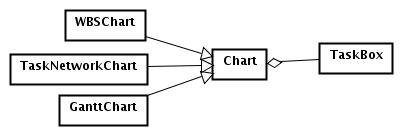
\includegraphics[width=0.6\textwidth]{../Milestone1-DomainModel/ChartDetail.png}
	\caption{chart and building blocks}
	\label{fig:chart} 
\end{figure}

Il \emph{Chart} modella il concetto di grafico generico. Per implementare la
specifica abbiamo queste specializzazioni:
\begin{itemize}
  \item \emph{GanttChart} che permette di avere la rappresentazione delle
  attivit\`a nel tempo
  \item \emph{WBSChart} per avere una vista gerarchica delle attivit\`a e di
  come sono state raffinate e decomposte in sotto attivit\`a
  \item \emph{TaskNetworkChart} per rappresentare le dipendenze di tipo
  \emph{finish-to start} fra coppie di attivit\`a
\end{itemize}

Per costruire un \emph{Chart} \`e sufficiente assemblare \emph{TaskBox} in base
ad alcune preferenze del client che richiede la generazione.
